% !TeX root = ../main.tex

\chapter{Methodology}\label{chapter:methodology}

This chapter presents the prediction, control, safety correction, and training methods used in this thesis. Based on the system model introduced in Chapter 3, this chapter further describes how these models are implemented in the code. The overall framework consists of an LSTM-based forecasting module, a pandapower-based simulation environment, a MADRL controller, a safety action projection mechanism, and EV constraint handling mechanism.

\section{Overall Framework}

The overall workflow can be summarized as follows. First, the historical data are processed into time-series sequences of load demand, PV generation, and electricity prices. The LSTM predictor then generates forecasts over a future prediction horizon. The environment constructs the observation by combining the current system state with the predicted sequences. Based on its own observation, each MADRL actor outputs a control action. The generated actions subsequently undergo local feasibility checks and, if enabled, a safety action projection procedure. The environment then updates the battery SoC, EV SoC, and the net load of each prosumer according to the final control actions. Next, pandapower performs the power flow calculation using the updated net loads. Finally, the environment computes the reward based on the electricity cost, EV charging requirements, battery behavior, and the distribution network operating condition, and returns the reward to the agents for training.
% 总体流程如下：首先将历史数据处理为负荷、光伏发电和电价时间序列，再由 LSTM 预测未来时域；环境结合当前状态与预测序列构建观测，各 MADRL 演员据此输出动作。动作经过局部可行性检查及可选的安全投影后，环境更新各产消者的电池 SoC、电动汽车 SoC 和净负荷，并由 pandapower 执行潮流计算。最后，环境根据电力成本、电动汽车需求、电池行为和配电网运行状态计算奖励并用于智能体训练。

Let \(x_t\) denote the external input data at the current time step, including load \(L_{i,t}\), PV generation \(G_{i,t}\), and electricity price \(p_t\). Let \(\hat{x}_{t:t+H-1}\) denote the prediction window of length \(H\). The process within a time step is given by
% 令 \(x_t\) 表示当前时间步的外部输入，包括负荷 \(L_{i,t}\)、光伏发电 \(G_{i,t}\) 和电价 \(p_t\)；令 \(\hat{x}_{t:t+H-1}\) 表示长度为 \(H\) 的预测窗口。单个时间步内的过程为：
\[
  x_t,\hat{x}_{t:t+H-1},SOC^b_t,SOC^{ev}_t
  \rightarrow
  o_t
  \rightarrow
  a_t
  \rightarrow
  \bar a_t
  \rightarrow
  s_{t+1},r_t.
\]
where \(o_t\) is the observation, \(a_t\) is the actor's raw action, \(\bar a_t\) is the executed action after feasibility checks or projection, \(s_{t+1}\) is the environment's next state, and \(r_t\) is the immediate reward for each agent.
% 其中，\(o_t\) 为观测，\(a_t\) 为演员的原始动作，\(\bar a_t\) 为经过可行性检查或投影后的执行动作，\(s_{t+1}\) 为环境下一状态，\(r_t\) 为各智能体的即时奖励。

The overall framework of this work includes the following steps:
% 本文总体框架包括以下步骤：
\begin{enumerate}
  \item Read historical household load, PV generation, and electricity price.
  % 读取历史家庭负荷、光伏发电和电价数据。
  \item Use LSTM model to generate future prediction sequences for electricity price, load, and PV generation.
  % 使用 LSTM 模型生成电价、负荷和光伏发电的未来预测序列。
  \item The environment constructs the observation based on the current SoC, EV connection status, current exogenous variables, and the prediction window.
  % 环境根据当前 SoC、电动汽车连接状态、当前外生变量和预测窗口构建观测。
  \item Each agent's actor outputs three action components: battery action, PV action, and EV action.
  % 各智能体的演员输出电池、光伏和电动汽车三个动作分量。
  \item The battery action is first mapped to the feasible power range of SoC; in projection-based variants, battery power and PV curtailment are further subjected to grid safety projection.
  % 电池动作先映射至 SoC 对应的可行功率范围；在投影控制器中，电池功率和光伏削减还需经过电网安全投影。
  \item The environment updates the battery SoC, EV SoC, PV utilization, and net load based on the final actions.
  % 环境根据最终动作更新电池 SoC、电动汽车 SoC、光伏利用量和净负荷。
  \item pandapower writes the prosumer net load to the low-voltage distribution network and performs power flow calculation.
  % pandapower 将产消者净负荷写入低压配电网并执行潮流计算。
  \item The environment calculates the reward based on economic terms, EV-related terms, battery-related terms, and grid safety terms.
  % 环境根据经济项、电动汽车项、电池项和电网安全项计算奖励。
  \item The transition is written to the replay buffer and is used to update the actor and critic networks.
  % 将转移样本写入经验回放缓冲区，用于更新演员和评论家网络。
\end{enumerate}

Figure~\ref{fig:methodology-framework} illustrates the main workflow of this work.
% 图~\ref{fig:methodology-framework} 展示了本文的主要工作流程。

\begin{figure}[htpb]
  \centering
  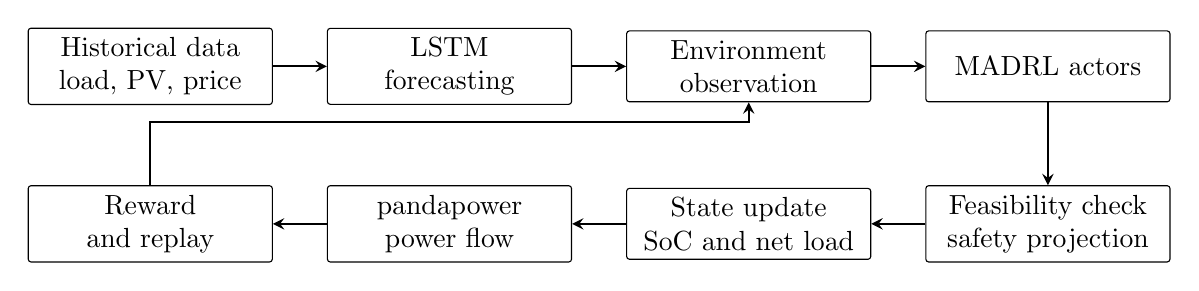
\begin{tikzpicture}[
    >=stealth,
    box/.style={draw, rounded corners=1pt, align=center, minimum width=31mm, minimum height=9mm},
    smallbox/.style={draw, rounded corners=1pt, align=center, minimum width=28mm, minimum height=8mm},
    arrow/.style={->, thick}
  ]
    \node[box] (data) at (0,1.6) {Historical data\\load, PV, price};
    \node[box] (lstm) at (3.8,1.6) {LSTM\\forecasting};
    \node[box] (obs) at (7.6,1.6) {Environment\\observation};
    \node[box] (actor) at (11.4,1.6) {MADRL actors};
    \node[box] (proj) at (11.4,-0.4) {Feasibility check\\safety projection};
    \node[box] (env) at (7.6,-0.4) {State update\\SoC and net load};
    \node[box] (pf) at (3.8,-0.4) {pandapower\\power flow};
    \node[box] (rew) at (0,-0.4) {Reward\\and replay};

    \draw[arrow] (data) -- (lstm);
    \draw[arrow] (lstm) -- (obs);
    \draw[arrow] (obs) -- (actor);
    \draw[arrow] (actor) -- (proj);
    \draw[arrow] (proj) -- (env);
    \draw[arrow] (env) -- (pf);
    \draw[arrow] (pf) -- (rew);
    \draw[arrow] (rew.north) -- ++(0,0.8) -| (obs.south);
  \end{tikzpicture}
  \caption{The work flow of the MADRL energy management framework.}\label{fig:methodology-framework}
\end{figure}

\section{LSTM Forecasting}

This thesis employs an LSTM forecasting module to provide future-horizon information to the controller. The forecasting targets include the electricity price, prosumer load, and PV generation. The prediction results determine the amount of future information available to the controller and can influence the scheduling performance of the stationary battery, PV curtailment, and EV charging.
% 本文采用基于 LSTM 的预测模块为控制器提供未来时域信息，预测对象包括电价、产消者负荷和光伏发电。预测结果决定控制器可获得的未来信息量，因而直接影响固定式电池、光伏削减和电动汽车充电的调度性能。

For any scalar sequence \(y_t\), LSTM uses a historical window of length \(h\) as input and outputs a predictive window of length \(H\). The current project configuration is
% 对任意标量序列 \(y_t\)，LSTM 以长度为 \(h\) 的历史窗口作为输入，并输出长度为 \(H\) 的预测窗口。当前配置为：
\[
  h=192,\qquad H=49.
\]
Since the simulation time step is 0.25 h, a historical window of 192 time steps corresponds to the previous 48 hours, while a prediction window of 49 time steps includes the current time step and approximately the following 12 hours. The training sample can be formulated as
% 仿真时间步为 \(0.25\ \mathrm{h}\)，因此 192 个历史时间步对应过去 48 小时，而 49 个预测时间步包含当前时刻及随后约 12 小时。训练样本可表示为：
\[
  X_k=(y_{k-h},y_{k-h+1},\ldots,y_{k-1}),
\]
\[
  Y_k=(y_k,y_{k+1},\ldots,y_{k+H-1}).
\]
The LSTM learns the mapping
% LSTM 学习以下映射：
\[
  \hat{Y}_k=f_{\theta}(X_k,\phi_k),
\]
where \(\phi_k\) denotes the optional temporal features, such as the hour of the day, the day of the week, or annual cyclic features.
% 其中，\(\phi_k\) 表示可选时间特征，例如日内小时、星期或年度周期特征。

In this work, the electricity price is predicted using a separate LSTM model; the PV generation is predicted using a shared model trained on reference PV sequences; and the load prediction is organized by prosumer and load components.
% 本文使用独立 LSTM 模型预测电价，使用基于参考光伏序列训练的共享模型预测光伏发电，并按产消者和负荷分量组织负荷预测。

The predicted sequences used in the environment are
% 环境中使用的预测序列为：
\[
  \hat p_{t:t+H-1},\qquad
  \hat L_{i,t:t+H-1},\qquad
  \hat G_{i,t:t+H-1}.
\]
In the perfect forecast mode, these sequences are directly obtained from the ground-truth future values. In the LSTM forecast mode, they are generated by the trained LSTM predictor. All the MADRL controller is trained using the LSTM forecast mode.

\section{MADRL Observation}

Observation of MADRL is divided into three components: the local observation, the forecast sequence observation, and the safety observation. This design follows the centralized training and decentralized execution (CTDE) paradigm. Specifically, each actor makes decentralized decisions based on its own local state and the forecast horizon, while the critic has access to the joint information of all agents during the training process.
% 观测由局部观测、预测序列观测和安全观测三部分组成。该设计遵循集中训练、分散执行（CTDE）范式：各演员主要依据自身局部状态和预测时域分散决策，而评论家在训练期间可以访问所有智能体的联合信息。

\subsection{Local Observation}

The local observation includes the physical states of each agent at the current time step:
% 局部观测包含各智能体在当前时间步的关键物理状态：
\[
  o^{local}_{i,t}
  =
  [SOC^b_{i,t},SOC^{ev}_{i,t},A^{ev}_t,L_{i,t},G_{i,t},p_t].
\]

In the MADRL actor, the local information is further transformed into \texttt{madrl\_local}. This feature includes intraday and annual cyclic time features, normalized battery SoC, normalized EV SoC, and EV availability indicators:
% 在 MADRL 演员中，局部信息进一步转换为 \texttt{madrl\_local}，其中包括日内和年度周期时间特征、归一化电池 SoC、归一化电动汽车 SoC 以及车辆可用性指标：
\[
\begin{aligned}
o^{madrl}_{i,t}
={}&[
\sin(2\pi \mathrm{hour}_t/24),
\cos(2\pi \mathrm{hour}_t/24),\\
&\sin(2\pi \mathrm{doy}_t/365.25),
\cos(2\pi \mathrm{doy}_t/365.25),\\
&\bar{SOC}^b_{i,t},
\bar{SOC}^{ev}_{i,t},
A^{ev}_t].
\end{aligned}
\]
This representation enables the actor not only to perceive the current states of the devices but also to identify the current temporal position within both the daily and annual cycles.
% 该表示使演员既能感知设备当前状态，也能识别当前时刻在日周期和年周期中的位置。

\subsection{Forecast Sequence Observation}

The forecast sequence observation describes the future trajectories of the electricity price, load demand, and PV generation. In the environment, the sequence can be expressed as
% 预测序列观测描述电价、负荷需求和光伏发电的未来轨迹。环境中的 \texttt{sequence} 可表示为：
\[
  o^{seq}_{i,t}
  =
  [\hat p_{t:t+H-1},\hat L_{i,t:t+H-1},\hat G_{i,t:t+H-1}].
\]
In practice, the MADRL actor uses normalized or relative representations of these forecast sequences:
% 实际应用中，MADRL 演员使用这些预测序列的归一化或相对表示：
\[
  \bar p_{t:t+H-1},\qquad
  \Delta \bar p_{t:t+H-1},\qquad
  \bar L_{i,t:t+H-1},\qquad
  \bar G_{i,t:t+H-1}.
\]
where \(\bar p\) denotes the relative electricity price within the prediction horizon, \(\Delta \bar p\) represents the price variation intensity over the prediction window, and \(\bar L\) and \(\bar G\) denote the normalized load and PV generation forecasts, respectively. Physically, these features enable the actor to schedule the stationary battery and EV charging according to anticipated periods of high or low electricity prices, while also determining whether battery capacity should be reserved or utilized based on the forecasted PV generation.
% 其中，\(\bar p\) 表示预测时域内的相对电价，\(\Delta\bar p\) 表示预测窗口内的电价变化强度，\(\bar L\) 和 \(\bar G\) 分别表示归一化负荷与光伏预测。这些特征使演员能够依据预期高低电价调度固定式电池和电动汽车充电，并根据光伏预测决定保留还是使用电池容量。

\subsection{Safety Observation}

The safety observation is used for feasibility checking and the safety projection procedure. It contains the physical parameters required to determine the device operating limits and perform the grid safety projection:
% 安全观测用于动作可行性检查和安全投影，包含确定设备运行边界及执行电网安全投影所需的物理参数：
\[
  o^{safe}_{i,t}
  =
  [SOC^b_{i,t},SOC^{ev}_{i,t},A^{ev}_t,L_{i,t},G_{i,t},
  C^b_i,P^{b,\max}_i,C^{ev}_i,P^{ev,\max}_i].
\]
Here, the battery capacity, battery maximum charging and discharging power, EV battery capacity, and EV maximum charging power directly determine the physically feasible action space. For example, the battery SoC together with \(P^{b,\max}_i\) determines the maximum amount of energy that can be charged into or discharged from the battery at the current time step. Similarly, the EV connection status together with \(P^{ev,\max}_i\) determines whether the EV is currently available for charging and, if so, the maximum allowable charging power.
% 电池容量与最大充放电功率、电动汽车电池容量与最大充电功率不仅是静态配置参数，也直接决定物理可行动作空间。例如，电池 SoC 与 \(P^{b,\max}_i\) 共同决定当前时间步可充入或放出的最大能量；车辆连接状态与 \(P^{ev,\max}_i\) 则决定当前能否充电及允许的最大充电功率。

\section{MADRL Action Design}

Each agent's actor outputs a three-dimensional action vector:
% 每个智能体的演员输出一个三维动作向量：
\[
  a_{i,t}=[a^b_{i,t},a^{pv}_{i,t},a^{ev}_{i,t}]\in[-1,1]^3.
\]
The three action components correspond to the stationary battery, PV utilization, and EV charging, respectively.
% 三个动作分量分别对应固定式电池、光伏利用和电动汽车充电。

\subsection{Battery Action Mapping}

The raw battery action generated by the actor is not executed directly as the physical battery power. Instead, it is first mapped to the feasible power range determined by the current battery SoC. Given the current SoC, the battery cannot be charged beyond \(SOC^b_{\max}\) or discharged below \(SOC^b_{\min}\) within a single time step. Therefore, the feasible battery power limits at the current time step are given by
% 演员生成的原始电池动作不会直接作为物理电池功率执行，而是先映射到由当前电池 SoC 决定的可行功率范围。电池在单个时间步内不能充电超过 \(SOC^b_{\max}\)，也不能放电低于 \(SOC^b_{\min}\)，因此当前时间步的可行电池功率边界为：
\[
  P^{b,low}_{i,t}
  =
  -\min
  \left(
  P^{b,\max}_i,
  \frac{(SOC^b_{i,t}-SOC^b_{\min})C^b_i\eta_b}{\Delta t}
  \right),
\]
\[
  P^{b,up}_{i,t}
  =
  \min
  \left(
  P^{b,\max}_i,
  \frac{(SOC^b_{\max}-SOC^b_{i,t})C^b_i}{\eta_b\Delta t}
  \right).
\]
The raw action \(a^b_{i,t}\in[-1,1]\) is linearly mapped to this interval:
% 原始动作 \(a^b_{i,t}\in[-1,1]\) 被线性映射至该区间：
\[
  P^b_{i,t}
  =
  P^{b,low}_{i,t}
  +
  \frac{a^b_{i,t}+1}{2}
  (P^{b,up}_{i,t}-P^{b,low}_{i,t}).
\]
This ensures that even if the actor outputs a boundary value, the executed action does not directly cause the battery SoC to violate its limits.
% 这确保即使演员输出边界值，执行动作也不会直接导致电池 SoC 越限。

\subsection{PV Action Mapping}

The PV action represents the PV utilization factor. It is defined as
% 光伏动作表示光伏利用系数，其定义为：
\[
  u^{pv}_{i,t}
  =
  \min
  \left(
  1,\max\left(0,\frac{a^{pv}_{i,t}+1}{2}\right)
  \right).
\]
The corresponding utilized PV generation and curtailed PV power are given by
% 相应的已利用光伏功率和削减光伏功率为：
\[
  G^{use}_{i,t}=u^{pv}_{i,t}G_{i,t},
\]
\[
  G^{curt}_{i,t}=G_{i,t}-G^{use}_{i,t}.
\]
When \(a^{pv}_{i,t}=1\), the agent uses all available PV; when \(a^{pv}_{i,t}=-1\), the PV is completely curtailed. The physical meaning of the PV action is to reduce reverse power flow or voltage violation risks through controllable curtailment.
% 当 \(a^{pv}_{i,t}=1\) 时，智能体利用全部可用光伏；当 \(a^{pv}_{i,t}=-1\) 时，光伏被完全削减。该动作的物理意义是通过可控削减降低反向潮流或电压越限风险。

\subsection{EV Action Mapping}

The EV action represents the utilization factor of the residential charger. It is defined as
% 电动汽车动作表示住宅充电桩利用系数，其定义为：
\[
  u^{ev}_{i,t}
  =
  \min
  \left(
  1,\max\left(0,\frac{a^{ev}_{i,t}+1}{2}\right)
  \right).
\]
Then, EV charging power requested by the actor is
% 演员请求的电动汽车充电功率为：
\[
  P^{ev,rl}_{i,t}
  =
  A^{ev}_t u^{ev}_{i,t}P^{ev,\max}_i.
\]
If the EV is not connected, \(A^{ev}_t=0\), the EV charging power is alwayszero regardless of the action produced by the actor. Subsequently, the environment determines the final executed charging power \(P^{ev}_{i,t}\) by considering the EV SoC headroom as well as the hard projection or emergency charging mechanism, if enabled.
% 若电动汽车未连接，即 \(A^{ev}_t=0\)，无论演员输出何种动作，充电功率始终为零。随后，环境结合电动汽车 SoC 裕度以及启用时的硬投影或紧急充电机制，确定最终执行功率 \(P^{ev}_{i,t}\)。

\section{Reward Function Design}

The reward function combines the economic objective, EV mobility requirements, battery behavior, and grid safety. For each agent \(i\), the total reward consists of multiple components. Positive terms represent benefits or incentives, whereas negative terms represent costs or constraint violations.

\subsection{EV Charging Cost}

EV charging draws electrical energy from either the grid or local energy resources. Its economic cost is determined by the actual charging power and the electricity price. Let
\[
  \tilde p_t=p_t+\mu^{imp}
\]
denote the electricity price. The basic EV charging cost is then given by
\[
  \mathcal{C}^{ev}_{i,t}
  =
  w^{ev}_{cost}P^{ev}_{i,t}\tilde p_t\Delta t.
\]
The corresponding reward term is
\[
  r^{ev,cost}_{i,t}=-\mathcal{C}^{ev}_{i,t}.
\]
EV charging during high-price periods incurs higher costs, while charging during low-price periods is more economical.

% Modified: replace the code-derived term ``Costweight'' with readable academic terminology.
\subsection{EV Cost-Weight Modelling}

Experimental results show that using only the EV charging cost as the reward encourages overly conservative EV charging behavior, even during periods of low electricity prices. The parameter \(w^{ev}_{cost}\) is therefore introduced to adjust the relative importance of the EV charging cost in the MADRL reward function. In the current implementation, the soft and hard modes use the configuration parameter \texttt{ev\_charging\_cost\_weight}, whereas the emergency mode uses a fixed value of 1:
\[
w^{ev}_{cost}=
\left\{
\begin{array}{ll}
\texttt{ev\_charging\_cost\_weight}, & \mathrm{mode}\in\{\mathrm{soft},\mathrm{hard}\},\\
1, & \mathrm{mode}=\mathrm{emergency}.
\end{array}
\right.
\]
When \(w^{ev}_{cost}>1\), the agent places greater emphasis on avoiding costly EV charging during periods of high electricity prices. 

\subsection{EV Departure Penalty}

The EV departure requirement represents a physical mobility constraint, requiring the EV to reach the target SoC before departure. In the reward function, the departure penalty converts this requirement into a learning signal under the soft mode. The SoC deficit at the departure time step is defined as
\[
  g^{dep}_{i,t}
  =
  \max(0,SOC^{ev}_{req}-SOC^{ev}_{i,t+1}),
  \qquad t_d=t^{dep}.
\]
The corresponding penalty is
\[
  L^{ev,dep}_{i,t}
  =
  w^{ev}_{dep}(g^{dep}_{i,t})^2.
\]
This penalty is activated only at the departure time step. 

\subsection{EV Progress Penalty}

Experimental results indicate that applying the departure penalty only at the departure time step is still insufficient to consistently achieve the required departure SoC. To solve this problem, an additional progress penalty can be enabled in the soft EV experiments. This penalty provides a linear reference trajectory from the arrival SoC to the required departure SoC throughout the EV connection window. Let \(\alpha_t\in[0,1]\) denote the normalized progress within the current connection window. Then,
\[
  SOC^{ev,prog}_{t}
  =
  SOC^{ev}_{arr}
  +
  \alpha_t(SOC^{ev}_{req}-SOC^{ev}_{arr}).
\]
if the EV SoC falls below this reference trajectory, a penalty is applied to encourage the agent to gradually approach the departure target during the night connection window. The progress gap can be expressed as
\[
  g^{prog}_{i,t}
  =
  \max(0,SOC^{ev,prog}_{t}-SOC^{ev}_{i,t+1}),
\]
The corresponding penalty is
\[
  L^{ev,prog}_{i,t}
  =
  w^{ev}_{prog}(g^{prog}_{i,t})^2.
\]
This term encourages the EV to gradually approach the required departure SoC throughout the overnight connection window, rather than postponing the entire charging demand until the final time steps before departure.

\subsection{Price-Aware Penalty}

During the experiments, it was further observed that increasing the EV costweight may cause competition between the EV reward and the battery reward. Moreover, the EV is still unable to completely avoid charging during periods of high electricity prices. To encourage the EV to avoid expensive charging periods, a price-aware penalty is introduced in this thesis. First, a quantile threshold is computed from the electricity price profile within the current episode:
\[
  p^{thr}=Q_q(\{p_{\tau}\}),
\]
where \(q\) denotes \texttt{ev\_price\_aware\_threshold\_quantile}, whose used value is 0.70. When the current electricity price exceeds this threshold, the normalized excess electricity price is defined as
\[
  \delta^p_t
  =
  \frac{\max(0,\tilde p_t-p^{thr})}{\max(p^{thr},10^{-6})}.
\]
The price-aware penalty is then defined as
\[
  L^{ev,price}_{i,t}
  =
  w^{ev}_{price}P^{ev}_{i,t}\delta^p_t\Delta t.
\]
When the electricity price does not exceed the threshold, this penalty is zero. When the electricity price exceeds the threshold and the EV is charging, this term becomes a positive penalty, encouraging the agent to shift flexible EV charging demand to periods with relatively lower electricity prices.

\subsection{Battery Reward and Regularization}

The battery reward consists of four components: the economic benefit of battery charging and discharging, the boundary action penalty, the SoC regularization term, and the throughput bonus applied during the early stage of training. The instantaneous economic benefit of the battery is given by
\[
  r^{bat}_{i,t}
  =
  [\max(-P^b_{i,t},0)-\max(P^b_{i,t},0)]
  \tilde p_t\Delta t.
\]
When the battery is already close to its SoC limits but continues to move toward the corresponding boundary, an action boundary penalty is imposed:
\[
  L^{bat,act}_{i,t}
  =
  w^{bat}_{act}|P^b_{i,t}|I^{bd}_{i,t}.
\]
where \(I^{bd}_{i,t}=1\) indicates that the battery is discharging near a low SoC limit or charging near a high SoC limit; otherwise, \(I^{bd}_{i,t}=0\). Additionally, the SoC regularization term encourages the battery to stay away from the hard limits:
\[
  L^{bat,soc}_{i,t}
  =
  w^{bat}_{soc}
  [
  \max(0,SOC^{soft}_{low}-SOC^b_{i,t})^2
  +
  \max(0,SOC^b_{i,t}-SOC^{soft}_{high})^2
  ].
\]
The throughput bonus for battery applied during the early stage of training is given by
\[
  r^{bat,thr}_{i,t}
  =
  w^{thr}_t |P^b_{i,t}|\Delta t.
\]
This term gradually decays with training progress, aiming to prevent the actor from learning overly conservative strategies that avoid using the battery entirely in the early stages of training.

\subsection{Grid Safety Penalty}

The grid safety penalty is derived from the results of the pandapower power flow calculation and consists of the three categories introduced previously: voltage violations, line loading violations, and transformer loading violations, as mentioned before. Let \(\psi^V_t\), \(\psi^{line}_t\), and \(\psi^{tr}_t\) denote the raw violation measures for voltage, line loading, and transformer loading, respectively. The corresponding penalty terms are
\[
  L^V_{i,t}=Nw_V\psi^V_t\omega^V_{i,t},
\]
\[
  L^{line}_{i,t}=w_{line}\psi^{line}_t,
\]
\[
  L^{tr}_{i,t}=w_{tr}\psi^{tr}_t.
\]
where \(\omega^V_{i,t}\) denotes the voltage penalty weight based on the degree of voltage violation for each agent bus; line and transformer penalties are currently the same for all agents. This design ensures that agents not only focus on their own economic benefits but also perceive the impact of their actions on the safety of the distribution grid.

\subsection{Total Reward}

The total reward for each agent can be written as
\[
\begin{array}{ll}
r_{i,t}={}&
r^{bat}_{i,t}
-\mathcal{C}^{ev}_{i,t}
-L^{bat,act}_{i,t}
-L^{bat,soc}_{i,t}
-L^{ev,dep}_{i,t}
-L^{ev,prog}_{i,t}\\[1mm]
&
-L^{ev,price}_{i,t}
-L^{ev,proj}_{i,t}
-L^{ev,eme}_{i,t}
+r^{bat,thr}_{i,t}
-L^V_{i,t}
-L^{line}_{i,t}
-L^{tr}_{i,t}.
\end{array}
\]
Here, \(L^{ev,proj}_{i,t}\) and \(L^{ev,eme}_{i,t}\) denote the diagnostic penalty terms introduced by the hard projection and emergency charging mechanisms, respectively, which will be discussed in the following sections. Overall, the reward function is designed to simultaneously encourage cost-efficient operation, satisfy the EV mobility requirements, promote appropriate battery utilization, and prevent violations of the distribution network safety constraints.

\section{Safety Projection for Grid Constraints}

The reward penalty represents a soft constraint: it allows the agent to take unsafe actions but penalizes such behavior through the reward function. In contrast, the safety projection acts as a hard correction mechanism applied before action execution. It directly modifies the control actions before they are executed by the environment, thereby moving them closer to the grid-safe feasible region. In the projection-based controllers, the safety projection is employed as a complement to the reward penalty mechanism.

\[
  x^{\mathrm{proj}}_t=
  [P^b_{1,t},\ldots,P^b_{N,t},
  G^{curt}_{1,t},\ldots,G^{curt}_{N,t}].
\]
Given the current load, PV generation, and EV charging power, the base net load is
\[
  P^{base}_{i,t}=L_{i,t}-G_{i,t}+P^{ev}_{i,t}.
\]
The safety projector uses pandapower to compute finite-difference sensitivities of the bus voltages and line loading with respect to the agents' net power injections around the zero-injection operating point. The corresponding linearized relationships can be written as
\[
  V_t \approx V^{base}+S^V\Delta P_t,
\]
\[
  \lambda^{line}_t \approx \lambda^{base}+S^{line}\Delta P_t.
\]
where \(\Delta P_t\) is determined by the battery power and PV curtailment. The projection goal is to satisfy the linearized safety constraints with respect to voltage, line, and transformer limits while making minimal changes to the original actions.

Each linearized constraint can be written in half-space form
\[
  r_j^T x^{\mathrm{proj}}_t \le b_j.
\]
If the current solution \(x^{\mathrm{proj}}_t\) violates the corresponding constraint, it is projected sequentially onto each constraint hyperplane as
\[
  x^{\mathrm{proj}}_t
  \leftarrow
  x^{\mathrm{proj}}_t
  -
  \frac{\max(0,r_j^Tx^{\mathrm{proj}}_t-b_j)}{\|r_j\|_2^2}r_j.
\]
After the projection step, the battery power is clipped again to the locally feasible SoC range, while the PV curtailment is clipped to
\[
  0\le G^{curt}_{i,t}\le G_{i,t}.
\]
This procedure is repeated for several iterations. Physically, the projection mitigates voltage and line loading violations by reducing battery charging, increasing battery discharging, or increasing PV curtailment. Since EV charging is primarily driven by the user's mobility requirements, this thesis treats the EV constraints separately from the grid safety projection.

\section{EV Departure Requirement Handling}

This thesis uses three methods for handling the EV departure requirement: the soft, hard, and emergency charging strategies. All three approaches employ the same physical EV model, but they differ in terms of action execution and reward feedback.

\subsection{Soft Mode}

Soft mode directly executes the EV charging power requested by the actor, and guides policy learning through departure penalties, progress penalties, or costweight penalties in the reward function. The executed power is
\[
  P^{ev}_{i,t}=P^{ev,rl}_{i,t}
\]
and is subject to constraints from EV connection, charger power, and SoC headroom. 

\subsection{Hard Mode}

In the hard mode, the execution layer checks whether the current EV charging action is sufficient to preserve the feasibility of meeting the required departure SoC. Let \(K^{future}_t\) denote the number of remaining time steps during which the EV will remain connected before departure. The maximum achievable increase in SoC over the remaining connection window is
\[
  \Delta SOC^{future,\max}_{i,t}
  =
  \frac{K^{future}_tP^{ev,\max}_i\Delta t\eta_{ev}}{C^{ev}_i}.
\]
If the EV is not charged sufficiently at the current time step, it may become impossible to reach \(SOC^{ev}_{req}\) before departure, even if the charger subsequently operates at its maximum power. Therefore, the hard mode computes the minimum required charging power at the current time step as
\[
  P^{ev,req}_{i,t}
  =
  \max
  \left(
  0,
  \frac{(SOC^{ev}_{req}-\Delta SOC^{future,\max}_{i,t}-SOC^{ev}_{i,t})C^{ev}_i}
  {\Delta t\eta_{ev}}
  \right).
\]
The finally executed charging power is then determined by
\[
  P^{ev}_{i,t}
  =
  \min
  \left(
  P^{ev,\max}_i,
  \max(P^{ev,rl}_{i,t},P^{ev,req}_{i,t})
  \right).
\]
The physical meaning is that the control policy is free to select a charging power higher than the minimum required value, but it is not allowed to choose a charging power below the minimum necessary level.

\subsection{Emergency Charging}

Emergency charging is designed to compensate for the potential SoC deficiency that may occur under the EV soft mode. It is activated only within an emergency window immediately before the EV departure time. Let the emergency window consist of \(K^{eme}\) time steps. When the EV enters the emergency window and its SoC remains below the required target, the system computes the required charging power based on the remaining SoC deficit:
\[
  E^{need}_{i,t}
  =
  \max(0,SOC^{ev}_{req}-SOC^{ev}_{i,t})C^{ev}_i,
\]
\[
  P^{ev,eme}_{i,t}
  =
  \min
  \left(
  P^{ev,\max}_i,
  \frac{E^{need}_{i,t}}{K^{rem}_t\Delta t\eta_{ev}}
  \right).
\]
The finally executed power is then determined by
\[
  P^{ev}_{i,t}
  =
  \max(P^{ev,rl}_{i,t},P^{ev,eme}_{i,t}).
\]
This mode performs emergency charging only when the departure time is approaching. Therefore, the emergency mode is simpler to implement, but it may result in a large concentration of charging power during the final stage before departure.

\section{MADRL Training Algorithm}

This thesis adopts a multi-agent actor-critic framework based on the centralized training and decentralized execution paradigm. Each agent is equipped with an independent actor:
\[
  a_{i,t}=\pi_i(o_{i,t};\theta_i),
\]
where \(o_{i,t}\) denotes the actor observation of agent \(i\). During training, a centralized critic is employed, which receives the observations and the actions of all agents:
\[
  Q_i(o_{1:N,t},a_{1:N,t};\phi_i).
\]
To reduce Q-value overestimation, the code employs twin critics for each agent:
\[
  Q_{i,1},\qquad Q_{i,2}.
\]

Replay buffer saves transition：
\[
  (o_t,a_t,R^{(n)}_t,o_{t+n},d_t),
\]
where \(R^{(n)}_t\) is the n-step return：
\[
  R^{(n)}_{i,t}
  =
  \sum_{k=0}^{n-1}\gamma^k r_{i,t+k}.
\]
Here, \(n=48\) corresponds to an accumulated reward over approximately 12 hours. The critic target is given by
\[
  y_{i,t}
  =
  R^{(n)}_{i,t}
  +
  \gamma^n(1-d_t)
  \min(Q'_{i,1}(o_{t+n},a'_{t+n}),Q'_{i,2}(o_{t+n},a'_{t+n})).
\]
Target actions are added with TD3-style target policy smoothing noise:
\[
  a'_{t+n}
  =
  \mathrm{guard}
  \left(
  \pi'(o_{t+n})+\epsilon
  \right).
\]
where \(\mathrm{guard}\) denotes the local SoC feasibility check and optional safety projection.

Critic loss is
\[
  L^Q_i
  =
  (Q_{i,1}(o_t,a_t)-y_{i,t})^2
  +
  (Q_{i,2}(o_t,a_t)-y_{i,t})^2.
\]
During the actor update, only the \(i\)-th action in the joint action vector is replaced:
\[
  a^{pol}_{i,t}=\mathrm{guard}(\pi_i(o_{i,t})),
\]
\[
  L^{\pi}_i
  =
  -Q_{i,1}(o_t,a_{1,t},\ldots,a^{pol}_{i,t},\ldots,a_{N,t}).
\]
Target network uses soft update:
\[
  \theta'_i\leftarrow(1-\tau_{\mathrm{soft}})\theta'_i+\tau_{\mathrm{soft}}\theta_i,
\]
\[
  \phi'_i\leftarrow(1-\tau_{\mathrm{soft}})\phi'_i+\tau_{\mathrm{soft}}\phi_i.
\]

During training, both exploration noise and feasible random exploration are employed. The former adds random perturbations to the actor output, while the latter samples locally feasible battery actions with a certain probability during the early stage of training, thereby helping the agent explore the feasible battery SoC operating region.

\subsection{Training Pseudocode}

The overall MADRL training procedure adopted in this thesis can be summarized by the following pseudocode:

\begin{enumerate}
  \item Initialize \(N\) actors, \(N\) twin critics, the corresponding target networks, and the replay buffer.
  \item Reset the parallel training environments and obtain the initial observations.
  \item For each environment step:
  \begin{enumerate}
    \item Each actor generates a raw action based on its current observation.
    \item Add exploration noise and perform the local feasibility check.
    \item If a projection-based controller variant is enabled, perform the safety projection.
    \item Execute the actions in the environment, update the battery SoC, EV SoC, and net load, and perform the power flow calculation using pandapower.
    \item The environment returns the reward, the next observation, and the done flag.
    \item Store the transition in the replay buffer and compute the \(n\)-step return.
    \item Once the replay buffer contains sufficient samples, draw a mini-batch to update the critics.
    \item Update the actors and target networks every predefined number of training steps.
  \end{enumerate}
  \item Repeat the above procedure until the specified number of training episodes is reached.
\end{enumerate}

\section{Baseline Controllers}

To evaluate the performance of the proposed MADRL approach, this thesis also implements optimization-based baseline controllers, including Local MPC and ADMM-MPC.

\subsection{Local MPC}

Local MPC solves an independent receding-horizon optimization problem for each prosumer. It optimizes its own battery operation, PV curtailment, and EV charging schedule over the prediction horizon. For prosumer \(i\), the primary decision variables of the Local MPC formulation include
\[
  c_{i,\tau},d_{i,\tau},G^{curt}_{i,\tau},P^{ev}_{i,\tau},E^b_{i,\tau},E^{ev}_{i,\tau}.
\]
where \(c\) and \(d\) denote the battery charging power and discharging power, respectively, with
\[
  P^b_{i,\tau}=c_{i,\tau}-d_{i,\tau}.
\]
Function for the battery is: 
\[
  E^b_{i,\tau+1}
  =
  E^b_{i,\tau}
  +
  \eta_b c_{i,\tau}\Delta t
  -
  \frac{d_{i,\tau}\Delta t}{\eta_b}.
\]
Function for the EV is:
\[
  E^{ev}_{i,\tau+1}
  =
  E^{ev}_{i,\tau}
  +
  \eta_{ev}P^{ev}_{i,\tau}\Delta t.
\]
Local net load is:
\[
  P^{net}_{i,\tau}
  =
  L_{i,\tau}-G_{i,\tau}+G^{curt}_{i,\tau}
  +c_{i,\tau}-d_{i,\tau}
  +P^{ev}_{i,\tau}.
\]
Local MPC objective function mainly minimizes the battery charging cost, discharging benefit, and EV charging cost:
\[
  \min
  \sum_{\tau}
  \tilde p_{\tau}\Delta t
  (c_{i,\tau}-d_{i,\tau}+P^{ev}_{i,\tau})
  +
  \epsilon_b\Delta t(c_{i,\tau}+d_{i,\tau})
  +
  w^{ev}_{dep}g_i^2.
\]
where \(\epsilon_b\) is a small throughput tie-breaker, used to avoid unnecessary simultaneous charging and discharging or equivalent solutions; \(g_i\) is the EV departure gap. The advantage of Local MPC is that it has a small problem size and fast solution time; its disadvantage is the lack of grid coordination across agents.

\subsection{ADMM-MPC}

ADMM-MPC introduces distributed coordination based onLocal MPC. It tends to constrain the impact of aggregated net load on transformers. Each agent still solves its local subproblem, but additionally introduces local net load contribution
\[
  q_{i,\tau}=\alpha_{i,\tau}P^{net}_{i,\tau}.
\]
Here, \(\alpha_{i,\tau}=1\). The global coordination objective is to ensure that all agents' contributions satisfy the transformer aggregation bounds:
\[
  -\bar P^{tr}
  \le
  \sum_i q_{i,\tau}
  \le
  \bar P^{tr}.
\]
ADMM adds a quadratic penalty term to the local objective function :
\[
  J_i^{ADMM}
  =
  J_i^{local}
  +
  \frac{\rho}{2}
  \|\alpha_iP^{net}_i-z_i+u_i\|_2^2.
\]
where \(z_i\) is the coordination variable, \(u_i\) is the scaled dual variable, and \(\rho\) is the ADMM penalty parameter. The solution process iterates between local optimization and aggregation projection:
\[
  z\leftarrow \Pi_{[-\bar P^{tr},\bar P^{tr}]}(q+u),
\]
\[
  u\leftarrow u+q-z.
\]
Compared with Local MPC, ADMM-MPC provides a certain degree of system-level coordination.

\subsection{Rule-Based Controller}

In addition to the two optimization-based baseline approaches described above, this thesis also implements a rule-based EV and battery controller as a simple reference method. This controller provides a baseline strategy that does not rely on either learning algorithms or optimization solvers. The implemented controller is denoted as \texttt{rule\_based\_ev\_with\_battery}.

The EV charging rule depends only on the EV connection status and whether the EV SoC has reached its upper limit. If the EV is not connected, no charging is performed. If the EV is connected and \(SOC^{ev}_{i,t}<SOC^{ev}_{\max}\), the EV is charged at the maximum charging power:
\[
P^{ev}_{i,t}=
\left\{
\begin{array}{ll}
P^{ev,\max}_i, & A^{ev}_t=1\ \mathrm{and}\ SOC^{ev}_{i,t}<SOC^{ev}_{\max},\\
0, & \mathrm{otherwise}.
\end{array}
\right.
\]
This EV rule represents a simple charging behavior: once the vehicle arrives home, it immediately charges at the maximum power of the residential charger until the EV SoC reaches the upper limit. In addition, the stationary battery is controlled by a price-threshold rule based on the current electricity import price and the quantiles of the training electricity price distribution. Let \(\tilde p_t\) denote the current electricity import price, and let \(p^{low}\) and \(p^{high}\) denote the lower and upper quantile thresholds of the electricity price series used during training:
\[
  p^{low}=Q_{q_{low}}(\tilde p^{train}),
\]
\[
  p^{high}=Q_{q_{high}}(\tilde p^{train}).
\]
Based on these two thresholds, the battery power is determined as
\[
P^b_{i,t}=
\left\{
\begin{array}{ll}
\alpha_c P^{b,\max}_i, & \tilde p_t\le p^{low},\\
-\alpha_d P^{b,\max}_i, & \tilde p_t\ge p^{high},\\
0, & p^{low}<\tilde p_t<p^{high}.
\end{array}
\right.
\]
where \(\alpha_c\in[0,1]\) and \(\alpha_d\in[0,1]\) denote the charging and discharging ratios, respectively. In the current implementation, both parameters are set to 1. Consequently, the battery is commanded to charge at its maximum power during low-price periods, discharge at its maximum power during high-price periods, and remain idle when the electricity price falls between the two thresholds. The resulting battery action is still processed by the battery SoC feasibility mapping in the environment. Therefore, even if the rule requests maximum charging or discharging power, the executed battery power will never violate the SoC limits \([SOC^b_{\min},SOC^b_{\max}]\).

The physical meaning of this controller is: electrical energy is stored during periods of low electricity prices and released during periods of high electricity prices, while EV charging follows a fixed immediate-charging rule. The controller requires neither future forecasts nor the solution of an optimization problem, resulting in a very low computational cost. Compared with the MADRL and MPC approaches, it serves as a baseline that requires neither learning nor optimization.
